\documentclass[10pt, a4paper,spanish]{article}
\usepackage[utf8]{inputenc}

\usepackage{varwidth}
\usepackage{graphicx}

\usepackage[T1]{fontenc} % Use 8-bit encoding that has 256 glyphs
\usepackage{microtype} % Slightly tweak font spacing for aesthetics

\usepackage[hmarginratio=1:1,top=32mm,columnsep=20pt]{geometry} % Document margins
\usepackage[hang, small,labelfont=bf,up,textfont=it,up]{caption} % Custom captions under/above floats in tables or figures
\usepackage{booktabs} % Horizontal rules in tables
\usepackage{float} % Required for tables and figures in the multi-column environment - they need to be placed in specific locations with the [H] (e.g. \begin{table}[H])
\usepackage{hyperref} % For hyperlinks in the PDF

\usepackage{lettrine} % The lettrine is the first enlarged letter at the beginning of the text
\usepackage{paralist} % Used for the compactitem environment which makes bullet points with less space between them

\usepackage{abstract} % Allows abstract customization
\renewcommand{\abstractnamefont}{\normalfont\bfseries} % Set the "Abstract" text to bold
\renewcommand{\abstracttextfont}{\normalfont\small\itshape} % Set the abstract itself to small italic text

\usepackage{titlesec} % Allows customization of titles
\renewcommand\thesection{\Roman{section}} % Roman numerals for the sections
\renewcommand\thesubsection{\Roman{subsection}} % Roman numerals for subsections
\titleformat{\section}[block]{\large\scshape\centering}{\thesection.}{1em}{} % Change the look of the section titles
\titleformat{\subsection}[block]{\large}{\thesubsection.}{1em}{} % Change the look of the section titles

\usepackage{fancyhdr} % Headers and footers
\pagestyle{fancy} % All pages have headers and footers
\fancyhead{} % Blank out the default header
\fancyfoot{} % Blank out the default footer
\fancyhead[C]{ Mayo 2016 $\bullet$ JumpVa $\bullet$ Informe Final} % Custom header text
\fancyfoot[RO,LE]{\thepage} % Custom footer text

%----------------------------------------------------------------------------------------
%	TITLE SECTION
%----------------------------------------------------------------------------------------

\title{\vspace{-15mm}\fontsize{24pt}{10pt}\selectfont\textbf{Informe Final}} % Article title

\author{
\large
\textsc{Alberto Amigo Alonso\textsubscript{20\%}}\\[2mm] % Your name
\textsc{Sergio Delgado Álvarez\textsubscript{20\%}}\\[2mm] % Your name
\textsc{Sergio García Prado\textsubscript{20\%}}\\[2mm] % Your name
\textsc{Oscar Fernández Angulo\textsubscript{20\%}}\\[2mm] % Your name
\textsc{Silvia Rodriguez Ares\textsubscript{20\%}}\\[2mm] % Your name
\normalsize Universidad de Valladolid \\ % Your institution
\vspace{-5mm}
}
\date{}

%----------------------------------------------------------------------------------------

\begin{document}

	\maketitle % Insert title

	\thispagestyle{fancy} % All pages have headers and footers

%----------------------------------------------------------------------------------------
%	ABSTRACT
%----------------------------------------------------------------------------------------

	\begin{abstract}
		\noindent Servicio web destinado a permitir a remitentes y destinatarios ofertar envíos para que los transportistas sean capaces de encontrarlos permitiendo a todos los usuarios monitorizarlos.
	\end{abstract}

%----------------------------------------------------------------------------------------
%	TEXT
%----------------------------------------------------------------------------------------

	\section{Justificación de la elección}

		\paragraph{}
		Como propuesta de proyecto de grupo se ha decidido continuar con la idea del servicio de transporte de paquetes por el reto que supone la implementación de la elevada cantidad de contenido dinámico. Este se encuentra en todo el proceso de creación de un nuevo envío por parte de un usuario, así como de la oferta de los transportistas y la elección del usuario de entre todas las ofertas.

		\paragraph{}
		El nombre elegido para el sistema será \textbf{JumpVa}

		\paragraph{}
		Los cambios que se han realizado desde la primera propuesta han sido tanto del modelo de negocio de la empresa como de la implementación del diseño del sitio web. En cuanto al modelo de negocio, se ha añadido el rol de cliente-remitente (no realiza un envio, sino que requiere de alguien le recoja un paquete y se lo envie). Los cambios sobre el diseño se pueden ver en el documento desarrollado, aunque se enumeran a continuación:

			\begin{enumerate}
				\item Se han unificado los roles de remitente y destinatario en cliente, que dependiendo del envío actuará como remitente o destinatario según sea conveniente.

				\item Se facilita a los transportistas las rutas de los envios por los que pueden pujar mediante mapas, para que puedan diseñar sus propias rutas de transporte y aprovechar el camino para realizar varios pedidos.

				\item Se diferencian más rotundamente los roles de transportista y cliente, especializando los comportamientos que pueden realizar cada uno.

				\item La página de inicio que se muestra a los usuarios es directamente el historial de envios que tienen pendientes/finalizados. Esto proporciona agilidad a los usuarios en la experiencia de navegación por la web.

				\item En el historial de envios se usa un código de colores para indicar de una forma visual el estado de los envios. Por ejemplo Verde - Envio completado con exito, Amarillo - Pendiente de asignación.

				\item Se pasa del modelo de tablas que representan cada envio por un modelo de tarjetas desplegables. Cada tarjeta desplegable puede albergar mucha mas infomación que la tabla, por lo que se comprime mas la información sin llegar a resultar un problema de navegación.

				\item Se incorpora la plataforma de marcado de hitos. Cuando un cliente realiza un pago, marca la acción para que el transportista sepa que debe verificarlo.
			\end{enumerate}



	\section{Descripción del Problema}

		\paragraph{}
		El transporte es una actividad del sector terciario, entendida como el desplazamiento de objetos o personas de un lugar (punto de origen) a otro (punto de destino) en un vehículo (medio o sistema de transporte) que utiliza una determinada infraestructura (red de transporte). Esta ha sido una de las actividades terciarias que mayor expansión ha experimentado a lo largo de los últimos dos siglos, debido a la industrialización; al aumento del comercio y de los desplazamientos humanos tanto a escala nacional como internacional; y los avances técnicos que se han producido y que han repercutido en una mayor rapidez, capacidad, seguridad y menor coste de los transportes. \cite{wikipedia_transporte}

		\paragraph{}
		Nosotros nos centraremos en el transporte de mercancías para la realización de esta propuesta. En este sector existen tres roles bien diferenciados: el \textbf{remitente}, el \textbf{transportista} y el \textbf{destinatario}. El modelo de negocio actual se basa en empresas intermediarias denominadas \textit{agencias de transporte} cuya labor es poner en contacto remitentes con transportistas que lleven la mercancía hasta su destino.

		\paragraph{}
		Dependiendo de la manera en que se contrate el transporte existen dos formas de pago: por parte del remitente, del destinatario. Actualmente el método más utilizado es el de pago por parte del destinatario pero existen casos especiales en los que no es así. También existen dos métodos de calcular el precio del transporte: aplicando una tarifa fija (lo cual muchas veces infla los costes de manera innecesaria) o por contra, teniendo en cuenta la distancia recorrida desde el origen hasta el destino. Uno de los problemas actuales es el de calcular penalizaciones y recompensas por el tiempo de transporte así como el periodo de tiempo que transcurre durante la carga y descarga de la mercancía.

		\paragraph{}
		La solución que se propone es la creación de un servicio encargado de conectar a transportistas con remitentes y destinatarios de manera eficiente y automática tratando de minimizar los costes entre intermediarios, dando lugar a un mayor beneficio para el transportista y un menor coste para el cliente. En la siguiente sección se describirá más detalladamente tanto las acciones como la descripción de cada uno de los usuarios objetivo.

		\paragraph{}
		Dado que el sistema tratará de llegar al mayor número de personas posibles trataremos de hacer que la interfaz de usuario sea lo más simple posible.
		Se pretende que los usuarios comprendan cómo utilizar el sistema sin importar su edad ni conocimientos informáticos ya que los sectores a los que va destinado el sistema son muy heterogéneos. Por tanto será un punto muy importante tratar de mostrar el mayor número información posible sin sacrificar la facilidad de uso.

		\paragraph{}
		El servicio seguirá una idea similar a la de Uber \copyright\  con el transporte de pasajeros pero aplicado al campo de las mercancías (siempre siguiendo la vigente normativa). Ya existen algunas start-ups que pretenden hacerse un hueco en este nicho de mercado entre las que destacan Convoy \copyright\ y Trucker Path \copyright\ las cuales se basan en una aplicación para sistemas móviles. \cite{expansion_uber_transporte}

		\paragraph{}
		Los usuarios del sistema podran realizar las siguientes acciones:

		\begin{itemize}

			\item Los usuarios se registran en el sistema diferenciando su rol (cliente o transportista)

			\item Los clientes pueden crear envíos en el sistema para que los transportistas les oferten un precio por llevarlo a cabo.

			\item Los clientes seleccionarán al transportista que deseen de entre los que hayan pujado por la oferta de envío.

			\item Una vez confirmado el envío los clientes pueden monitorizar el envío

			\item Los transportistas pueden buscar envíos aplicando los filtros que crean convenientes (localizacion, fecha, etc).

			\item Todos los usuarios del sistema pueden notificar sobre hitos sucedidos en los envíos así como introducir comentarios, lo que fomenta la retroalimentación entre los involucrados.

			\item Los clientes y transportistas tendrán acceso a estadísticas sobre envíos anteriores.


		\end{itemize}



	\section{Usuarios Objetivo}

		\paragraph{}
		Los usuarios objetivo del sistema se dividen en dos grupos bien diferenciados:

		\begin{itemize}


			\item{\textbf{Transportista}}

			\paragraph{}
			El transportista es la persona encargada de llevar el envío desde el lugar de origen hasta el de destino.

			\paragraph{}
			El sistema, por tanto, tendrá la labor de permitirle encontrar envíos que se ajusten a las requisitos que el transportista requiera como localización del punto de partida, del de llegada, fecha, tipo de transporte, etc. Una vez que el transportista encuentre un envío que pretenda realizar deberá fijar un precio por el cual estaría dispuesto a llevarlo a cabo. A partir de este punto deberá esperar la confirmación del cliente para dirigirse al punto de partida.

			\paragraph{}
			Además de esto, el sistema también ofrecerá al transportista la posibilidad de notificar hitos al cliente tales como que su envío a sufrido algún contratiempo o que se ha completado cierta distancia.

			\paragraph{}
			El transportista también tendrá la posibilidad de acceder a información de anteriores envíos así como estadísticas sobre los destinos y orígenes, zonas donde se le han aceptado pujas más altas, etc.


			\item{\textbf{Cliente}}
			\paragraph{}
			El rol de cliente es el cliente. Este será quien oferte envíos a realizar en el sistema. Dentro de este se agrupan los dos clientes implicados en ello, es decir, el remitente y el destinatario. Estos roles no son fijos sino que se fijarán en cada envío según sea pertinente.

			\paragraph{}
			No existe restricción acerca de quién de los dos es el encargado de crear el envío, sino que habrá casos en los cuales serán los remitentes los que deseen enviar algo. También habrá casos en los cuales el destinatario es quien solicitará que se vaya a recoger mercancia a un lugar concreto.

			\paragraph{}
			El cliente que introduzca el envío en el sistema será también el encargado tanto de realizar el pago como de seleccionar el transportista que más desee de entre los que hayan pujado.

			\paragraph{}
			Ahora describiremos más detalladamente cada uno de los subroles:

			\begin{itemize}

				\item{\textbf{Remitente}}
				\paragraph{}
				El remitente será la persona encargada de suministrar la mercancia al transportista para que la lleve hasta el destinatario. El remitente podrá fijar una hora preferida de recogida dado que podría no estar disponible cuando el transportista llegue a recogerlo.

				\item{\textbf{Destinatario}}
				\paragraph{}
				El destinatario será la persona encargada de recoger el envío en el lugar de destino al cual llegará el transportista. El destinatarío podrá fijar una hora preferida de entrega dado que podría no estar disponible cuando el transportista llegue a entregarlo.

			\end{itemize}





		\end{itemize}
	\section{Borrador de la Solución}

		\paragraph{}
		La estructura de navegación por la página web será de scroll infinito siguiendo la idea que actualmente están llevando a cabo las principales redes sociales como Facebook \copyright y  Twitter \copyright. Hemos escogido esta idea en vez de la navegación por pestañas de la propuesta individual porque creemos que será más sencillo de utilizar para la mayoría de los usuarios.

		\paragraph{}
		A continuación procederemos a describir el conjunto de vistas que formarán el servicio web. Dado que existen dos roles bien diferenciados (cliente y transportista) las vistas que sean comunes a los dos pero tengan pequeñas diferencias se describirán juntas explicando dichas variaciones.

		\begin{figure}[H]
			\centering
			\begin{minipage}[b]{0.8\textwidth}
				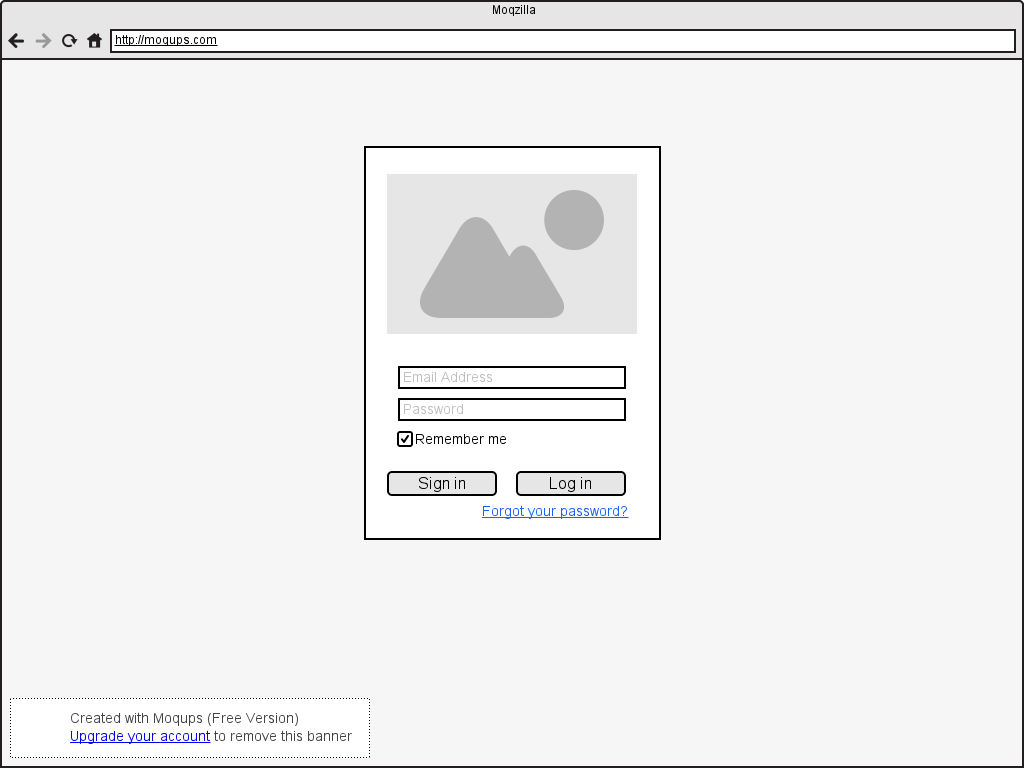
\includegraphics[width=\textwidth]{res/Login.png}
			\end{minipage}
		\end{figure}

		\paragraph{}
		La vista de \textbf{login} será lo primero que el usuario visualizará al acceder al sitio web, en esta parte se identificará o creará una cuenta en el caso de que no la tuviera todavía.


		\begin{figure}[H]
			\centering
			\begin{minipage}[b]{0.49\textwidth}
				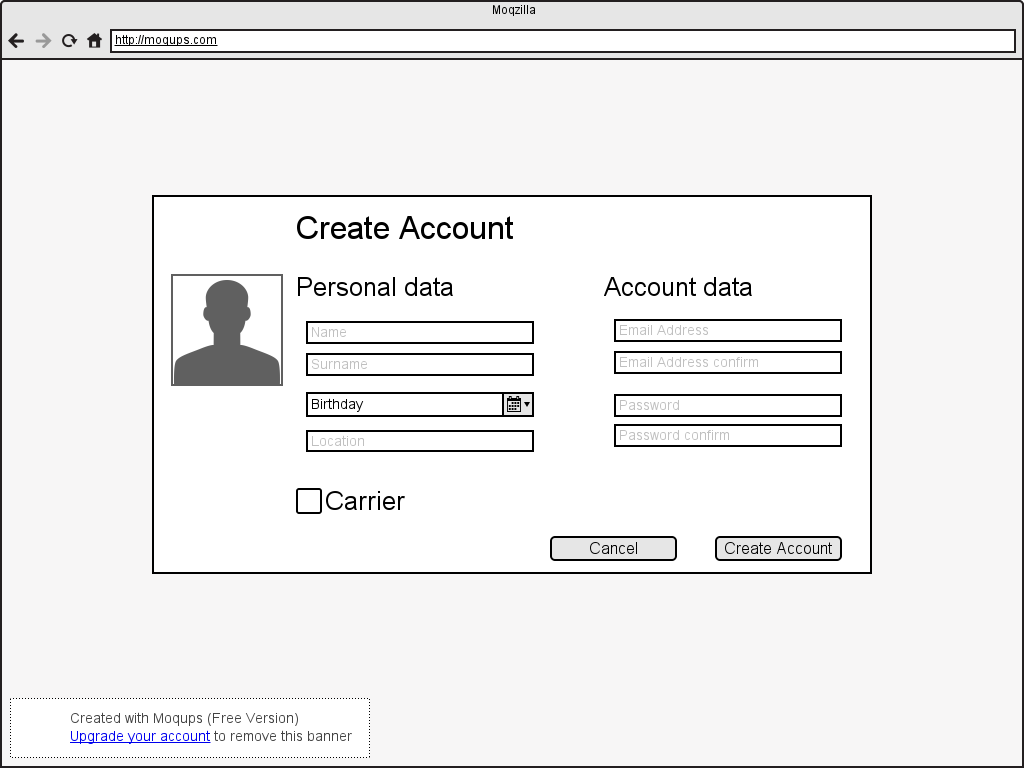
\includegraphics[width=\textwidth]{res/CrearCuenta.png}
			\end{minipage}
			\begin{minipage}[b]{0.49\textwidth}
				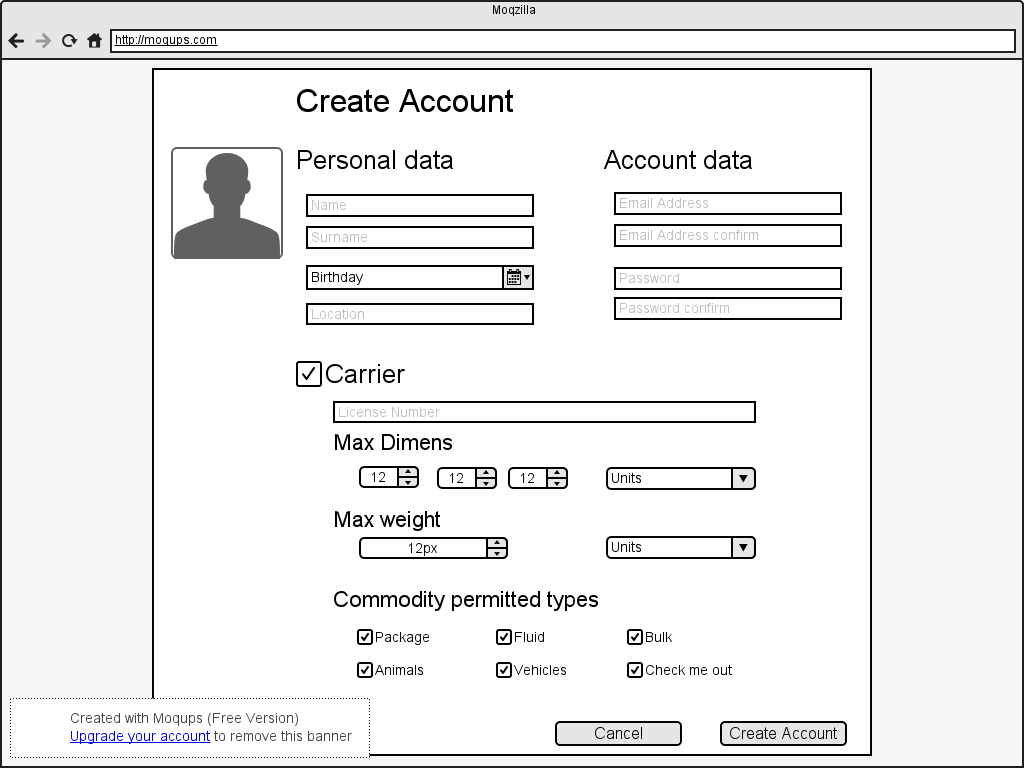
\includegraphics[width=\textwidth]{res/CrearCuentaTransportista.png}
			\end{minipage}
		\end{figure}

		\paragraph{}
		En la vista de \textbf{crear cuenta} es donde el usuario introducirá sus datos personales. Esta parte será común para los dos roles. Además habrá un checkbutton que el usuario deberá marcar en el caso de que sea transportista. Entonces en la vista aparecerán nuevos campos donde este deberá introducir las caracteristicas de su método de transporte (tamaño, peso máximo, tipo de envíos que puede transportar, etc). En este punto el sistema ya tendrá diferenciados los dos roles.

		\paragraph{}
		Primero describiremos las vistas que el cliente podrá visualizar y luego nos centraremos en las del transportista.

		\begin{figure}[H]
			\centering
			\begin{minipage}[b]{0.8\textwidth}
				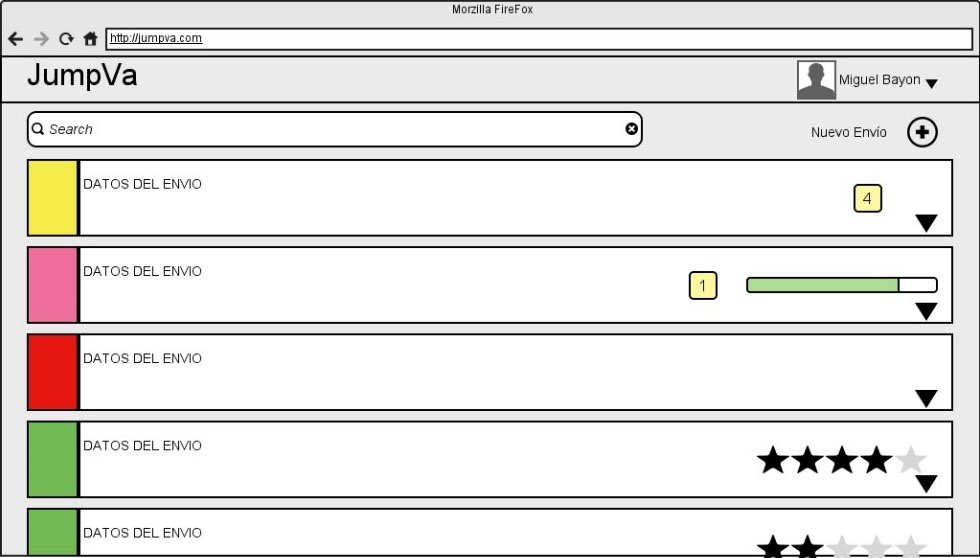
\includegraphics[width=\textwidth]{res/PaginaPrincipal.png}
			\end{minipage}
		\end{figure}

		\paragraph{}
		La vista de \textbf{página principal} del sitio web. Será la que se mostrará al iniciar sesión como remitente en el sitio web. En ella se mostrará al cliente información acerca de los envíos que están en curso, los que están pendientes de confirmación para que los confirme seleccionando el transportista que más desee. También se le mostrarán los envíos ya finalizados para que si lo desea pueda introducir la opinión acerca de anteriores envíos. Esta página tendrá un scroll infinito en el cual se le mostrarán todos los envíos que ha realizado. Además en la parte superior de la página habrá una barra de búsqueda que permitirá filtrar envíos por origenes, destinos, fechas, etc. lo cual permitirá encontrar cualquier envío anterior de manera sencilla. También hay un botón en la parte superior derecha cuya función es la de crear nuevos envíos.


		\begin{figure}[H]
			\centering
			\begin{minipage}[b]{0.49\textwidth}
				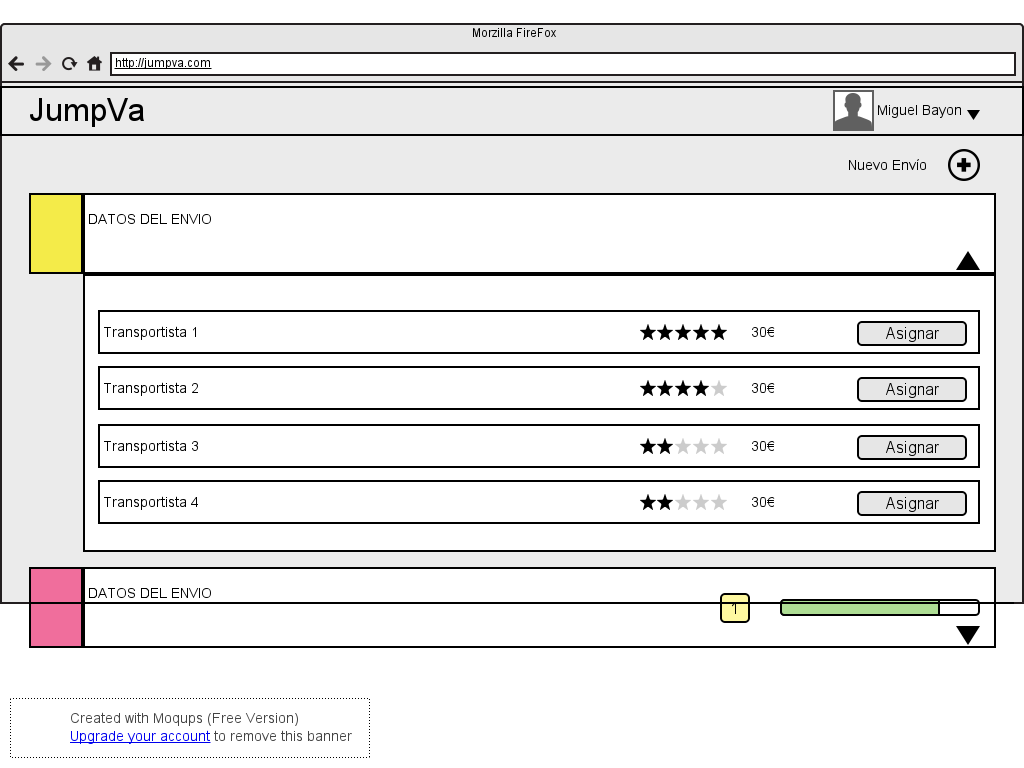
\includegraphics[width=\textwidth]{res/ExpansionEnvioPendienteAsignacion.png}
			\end{minipage}
			\begin{minipage}[b]{0.49\textwidth}
				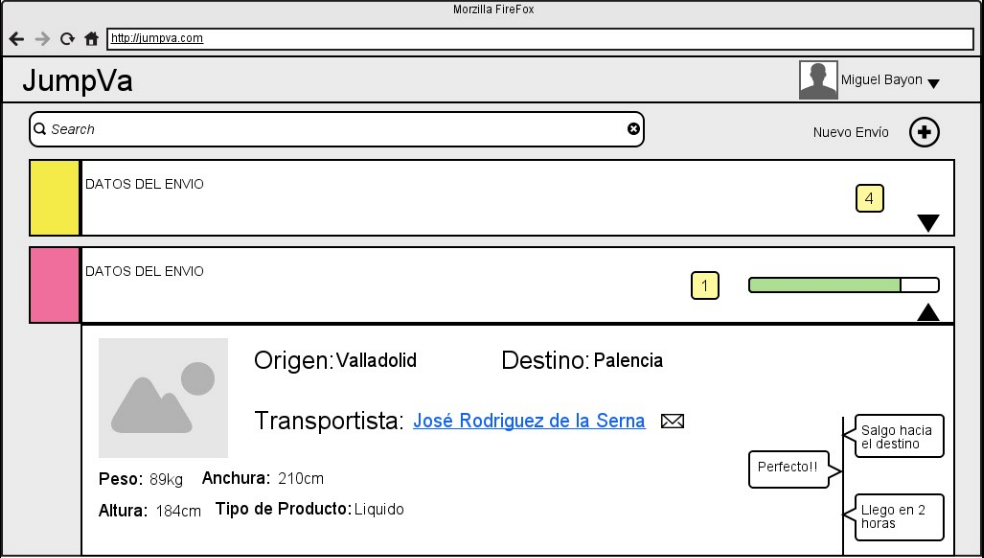
\includegraphics[width=\textwidth]{res/ExpansionEnvioEnProceso.png}
			\end{minipage}
		\end{figure}

		\paragraph{}
		Las dos vistas que se adjuntan en la imagen superior se corresponden con la información que se muestra al clickar (se abre un menu desplegable inferiormente) en los envíos que todavía no están confirmados, y un envío en progreso, este ultimo sera comun para ambos tipos de usuario.


		\begin{figure}[H]
			\centering
			\begin{minipage}[b]{0.49\textwidth}
				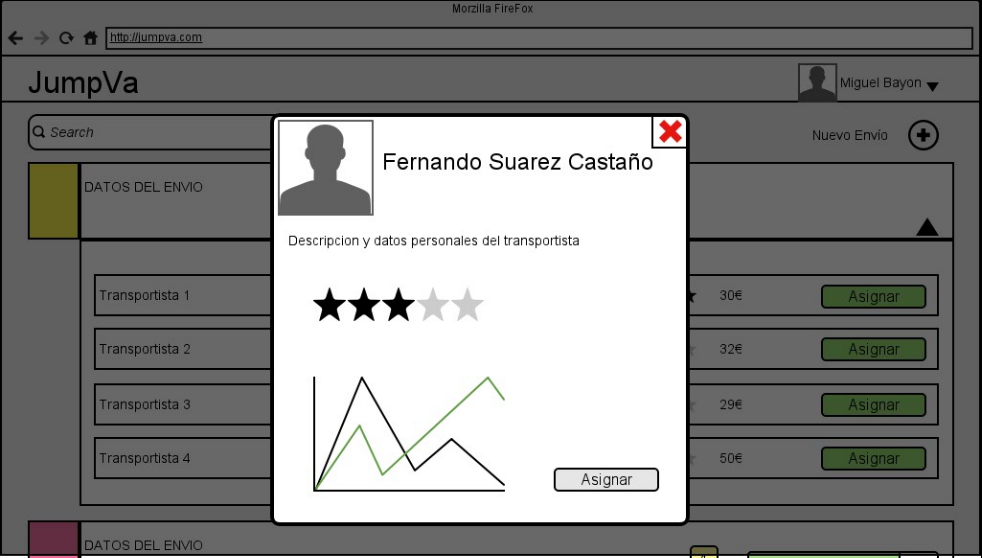
\includegraphics[width=\textwidth]{res/DetallesTransportista.png}
			\end{minipage}
			\begin{minipage}[b]{0.49\textwidth}
				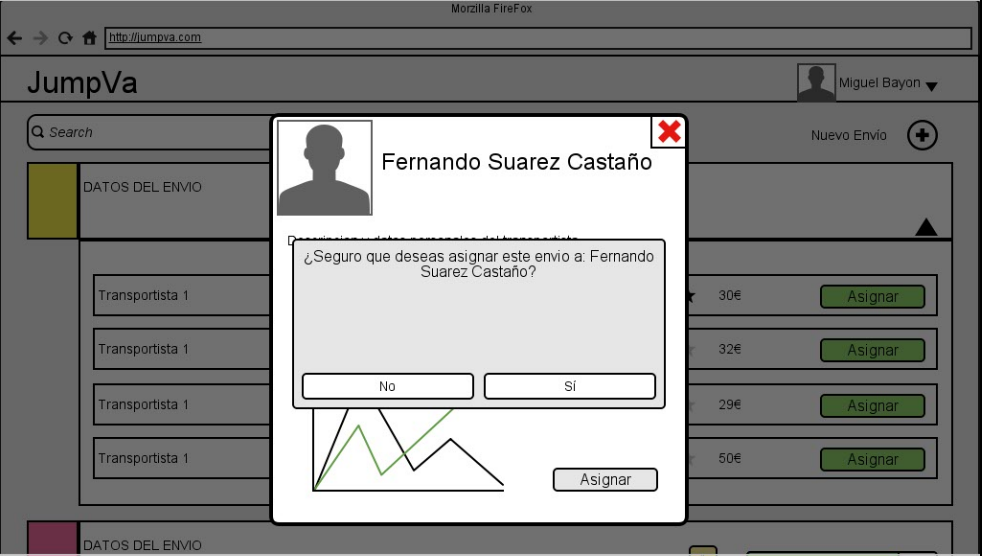
\includegraphics[width=\textwidth]{res/ConfirmacionAsignacion.png}
			\end{minipage}
		\end{figure}

		\paragraph{}
		La imagen superior ilustra el caso de que un cliente consulte el perfil de un transportista y seguidamente quiera confirmar que lo realice ese transportista.

		\begin{figure}[H]
			\centering
			\begin{minipage}[b]{0.49\textwidth}
				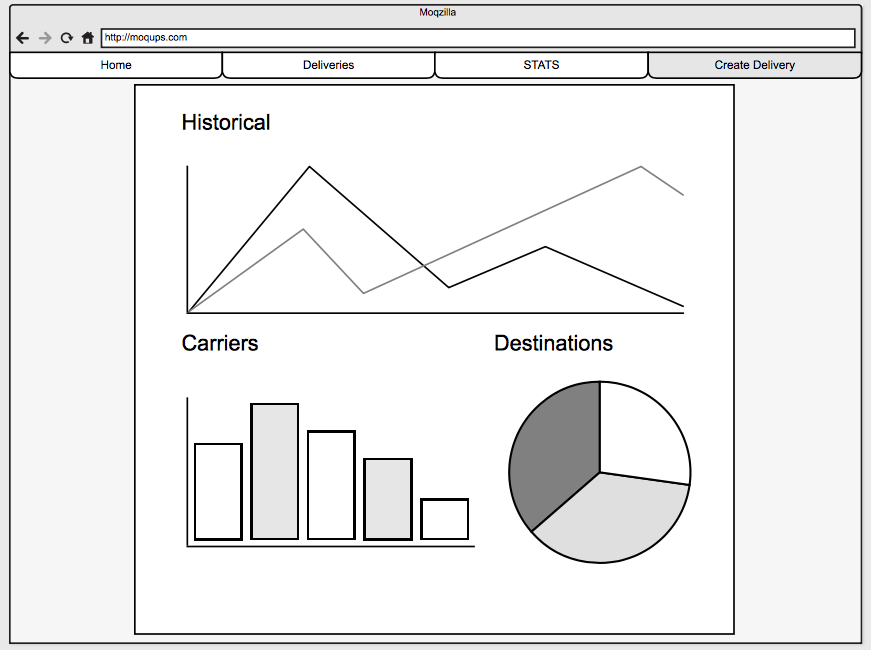
\includegraphics[width=\textwidth]{res/Estadisticas.png}
			\end{minipage}
			\begin{minipage}[b]{0.49\textwidth}
				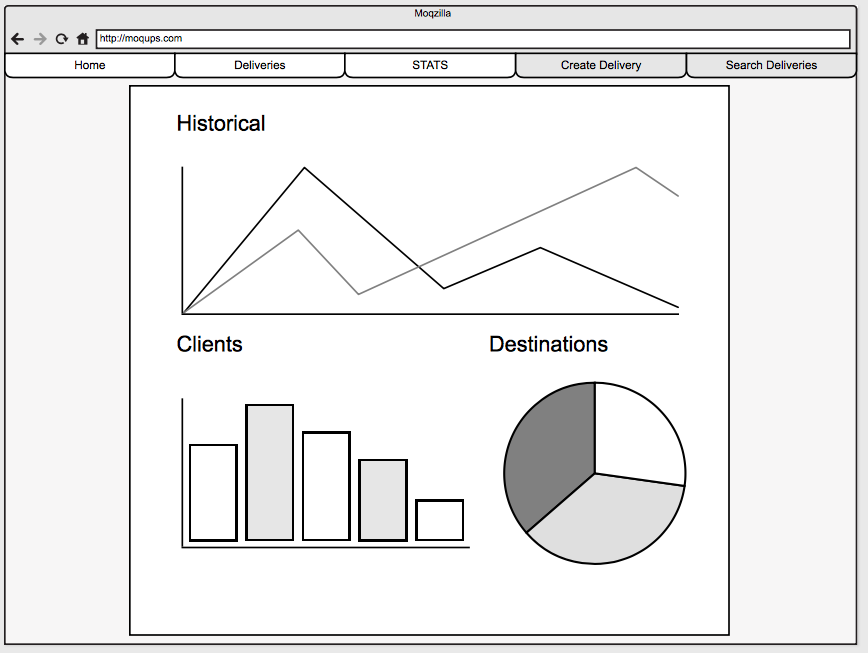
\includegraphics[width=\textwidth]{res/EstadisticasTransportista.png}
			\end{minipage}
		\end{figure}

		\paragraph{}
		La vista de \textbf{estadisticas} servirá para que los usuarios puedan obtener información gráficamente de manera rápida sobre envíos pasados. Tendrán un gráfico de líneas en el cual se mostrará la evolución del número de envíos respecto del tiempo. Además también tendrán otras métricas como el número de veces que han usado el mismo transportista en el caso del cliente y a la inversa en el caso del transportista. También podrán obtener métricas acerca de los orígenes y destinos a los que se han enviado pedidos, etc.

		\paragraph{}
		Las siguientes vistas serán de tipo emergente, es decir, se superpondrán al resto del contenido de la página. Si es posible se intentará hacer sin utilizar ventanas.


		\begin{figure}[H]
			\centering
			\begin{minipage}[b]{0.7\textwidth}
				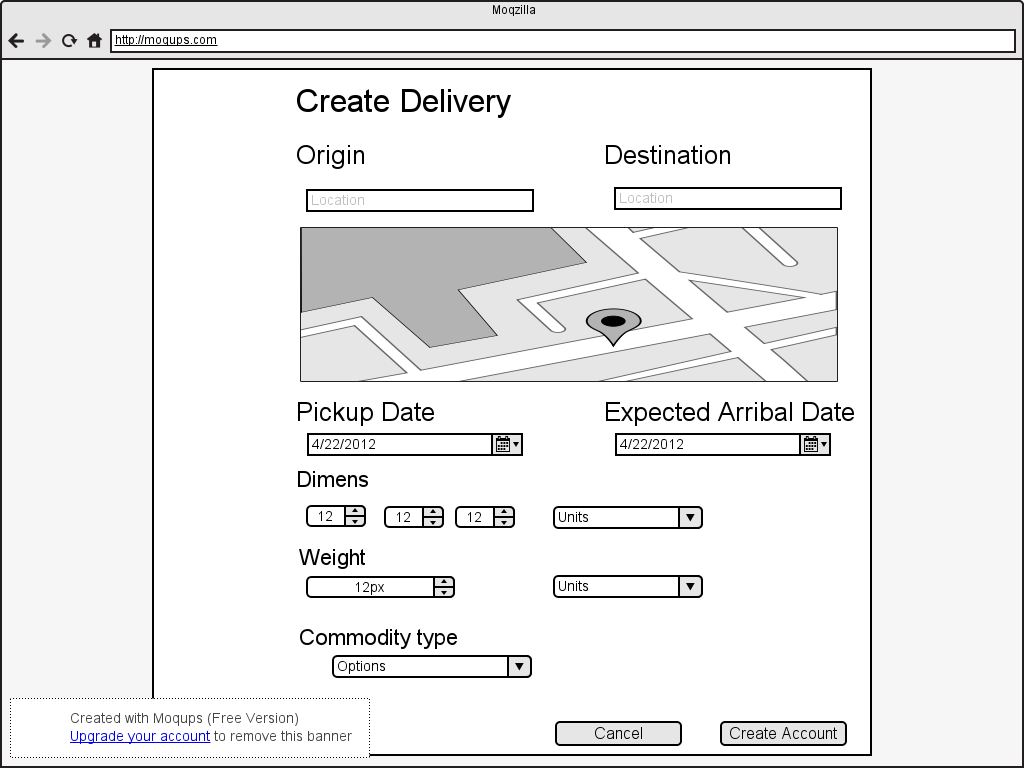
\includegraphics[width=\textwidth]{res/CrearEnvio.png}
			\end{minipage}
		\end{figure}

		\paragraph{}
		La vista de \textbf{crear envío} será única para los clientes. En esta introducirán información acerca de qué quieren enviar, desde dónde hasta dónde, en qué fecha, etc. El cliente además tendrá la posibilidad de introducir imágenes del paquete que después el transportista podrá visualizar antes de solicitar realizar el envío.

		\begin{figure}[H]
			\centering
			\begin{minipage}[b]{0.7\textwidth}
				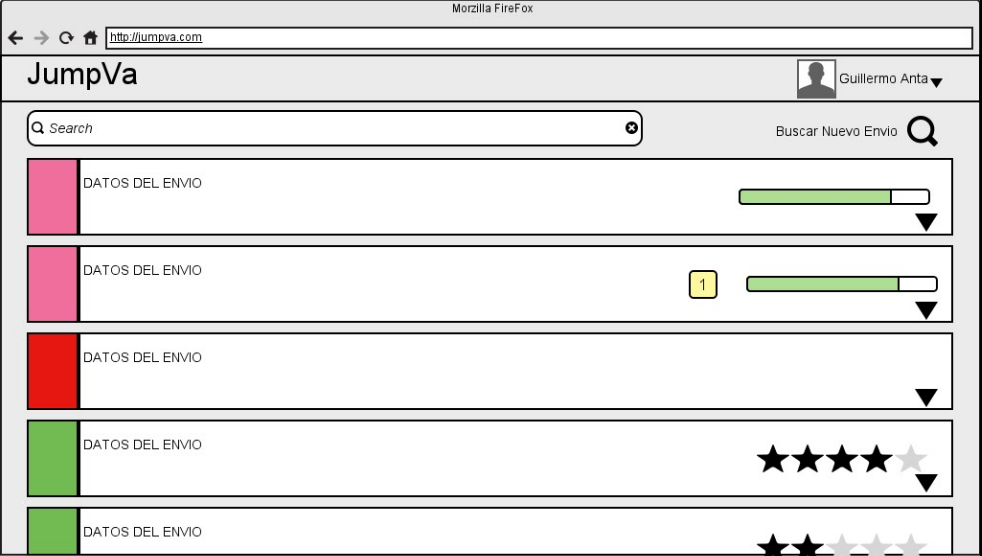
\includegraphics[width=\textwidth]{res/PaginaPrincipalTransportista.png}
			\end{minipage}
		\end{figure}

		\paragraph{}
		La vista de \textbf{pagina principal transportista}, sera la pagina principal que se visualizara al iniciar sesion como transportista. Es muy similar a la pagina principal del remitente. En ella el cliente podra consultar todos los envios que esta realizando en este momento, los que ya ha completado... Tambien tendra la posibilidad de buscar un nuevo envio si asi lo desea. Las vistas que se mostraran al hacer click sobre los diferentes envios que aparecen en la pagina principal seran similares a las descritas anteriormente.


		\begin{figure}[H]
			\centering
			\begin{minipage}[b]{0.7\textwidth}
				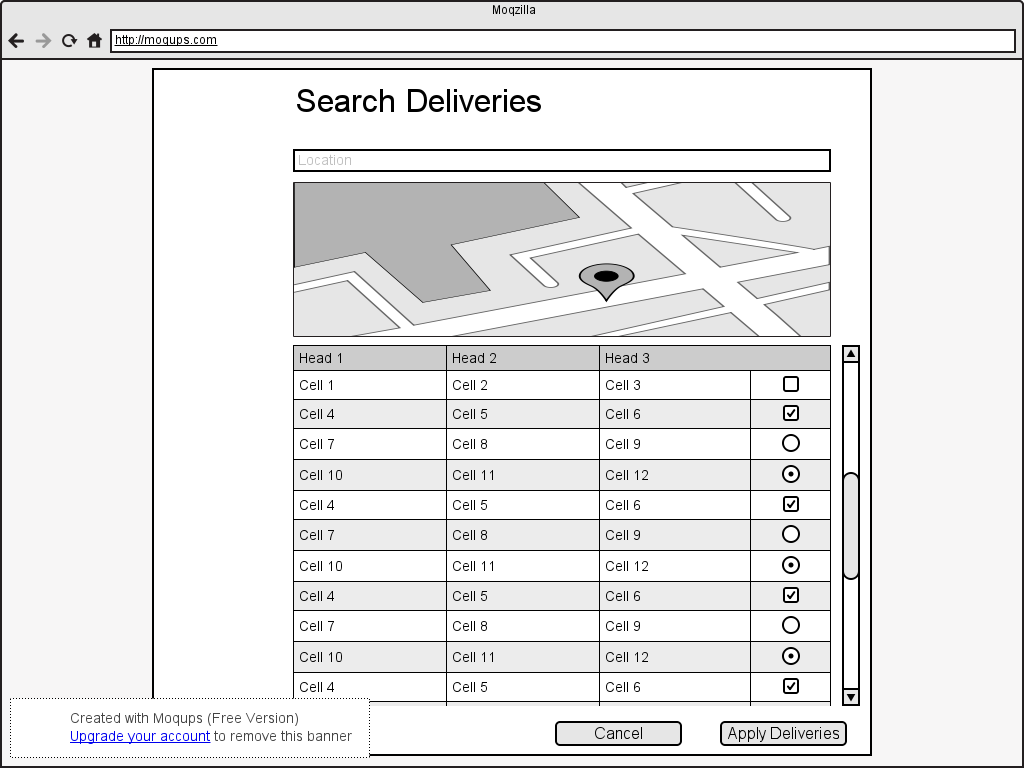
\includegraphics[width=\textwidth]{res/BuscarEnviosTransportista.png}
			\end{minipage}
		\end{figure}

		\paragraph{}
		La vista de \textbf{buscar envíos} será única para los transportistas. En esta vista los transportistas introducirán su ubicación actual o utilizaran la barra de busqueda y seguidamente el sistema les devolverá un listado los envíos disponibles más cercanos. Seguidamente el transportista podrá revisar la informacion de los diferentes envios, y si lo desea pujar por aquellos que le interesen.


		\begin{figure}[H]
			\centering
			\begin{minipage}[b]{0.49\textwidth}
				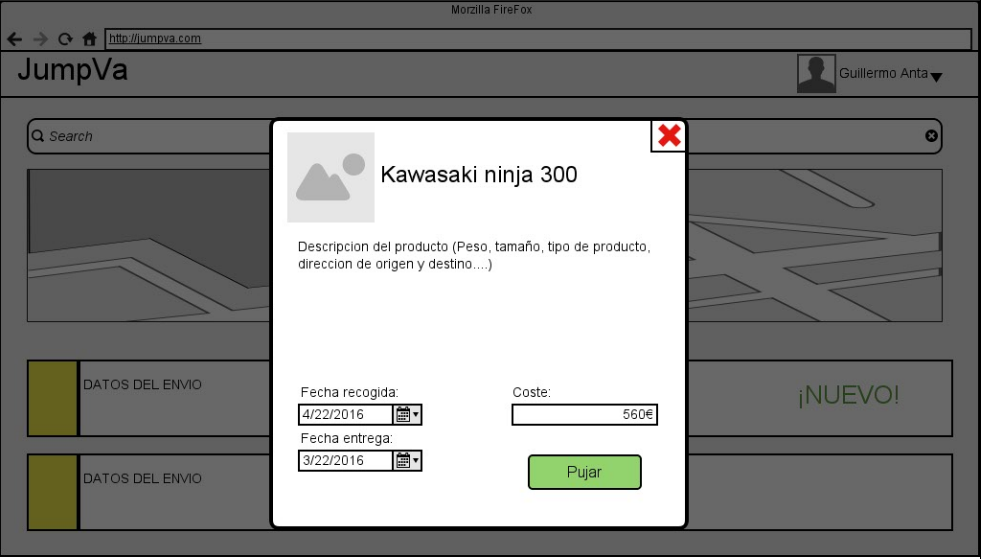
\includegraphics[width=\textwidth]{res/DetallesDeEnvio.png}
			\end{minipage}
			\begin{minipage}[b]{0.49\textwidth}
				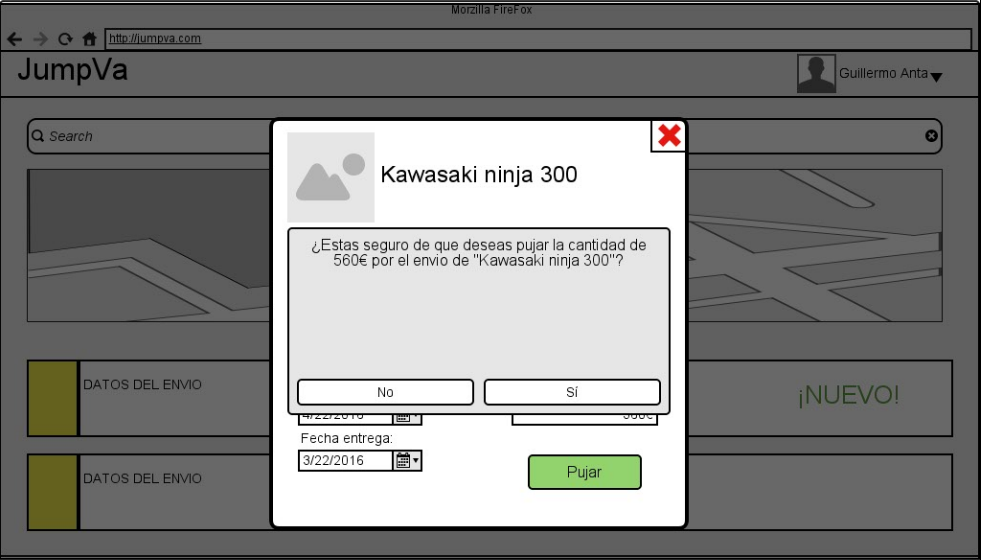
\includegraphics[width=\textwidth]{res/ConfirmacionDePuja.png}
			\end{minipage}
		\end{figure}

		\paragraph{}
		La vista de \textbf{envío} se corresponde con la informacion mostrada al hacer click sobre uno de los envios que aparecen listados en la página de busqueda, y en ella el transportista podra realizar una oferta para realizar el envio. La vista de \textbf{confirmar puja} se mostrara para confirmar que la puja introducida por el transportista es la deseada.

		\paragraph{}
		Ambas vistas seran de tipo emergente, se superpondran al resto del contenido dejandolo oscurecido en un segundo plano.

	\section{Especificación de requisitos:}

		\paragraph{}
		Requisitos funcionales: El sistema deberá...

			\begin{itemize}
				\item registrar nuevos usuarios.
				\item crear un nuevo envío.
				\item buscar un envío en su historial.
				\item cambiar el estado de los envíos.
				\item permitir al usuario puntuar los envíos.
				\item guardar un historial de los envíos (información).
				\item permitir a los usuarios consultar el estado de los envíos.
				\item actualizar el progreso de los envíos.
				\item permitir a los transportistas pujar por un envío.
				\item permitir a los transportistas añadir hitos a un envío.
				\item asegurar que todos los usuarios están previamente identificados en el sistema para poder acceder a cualquier función.
				\item notificar al usuario nuevas incidencias en los envíos.
				\item permitir a los remitentes consultar el historial de los transportistas relacionados con el envío.
				\item permitir a los remitentes puntuar al transportista que ha realizado su envío.
				\item permitir a los transportistas realizar una oferta para un evento.
				\item pedir una confimación para realizar una oferta.
				\item pedir una confimación para asignar un envío.
				\item permitir al transportista buscar nuevos envíos.
			\end{itemize}

			\paragraph{}
			Requisitos no funcionales: El sistema deberá...

				\begin{itemize}
					\item usar una base de datos como medio de almacenamiento.
					\item permitir hacer login a los usuarios que están en la base de datos.
				\end{itemize}
	\section{Casos de uso:}


		\begin{figure}[H]
			\centering
				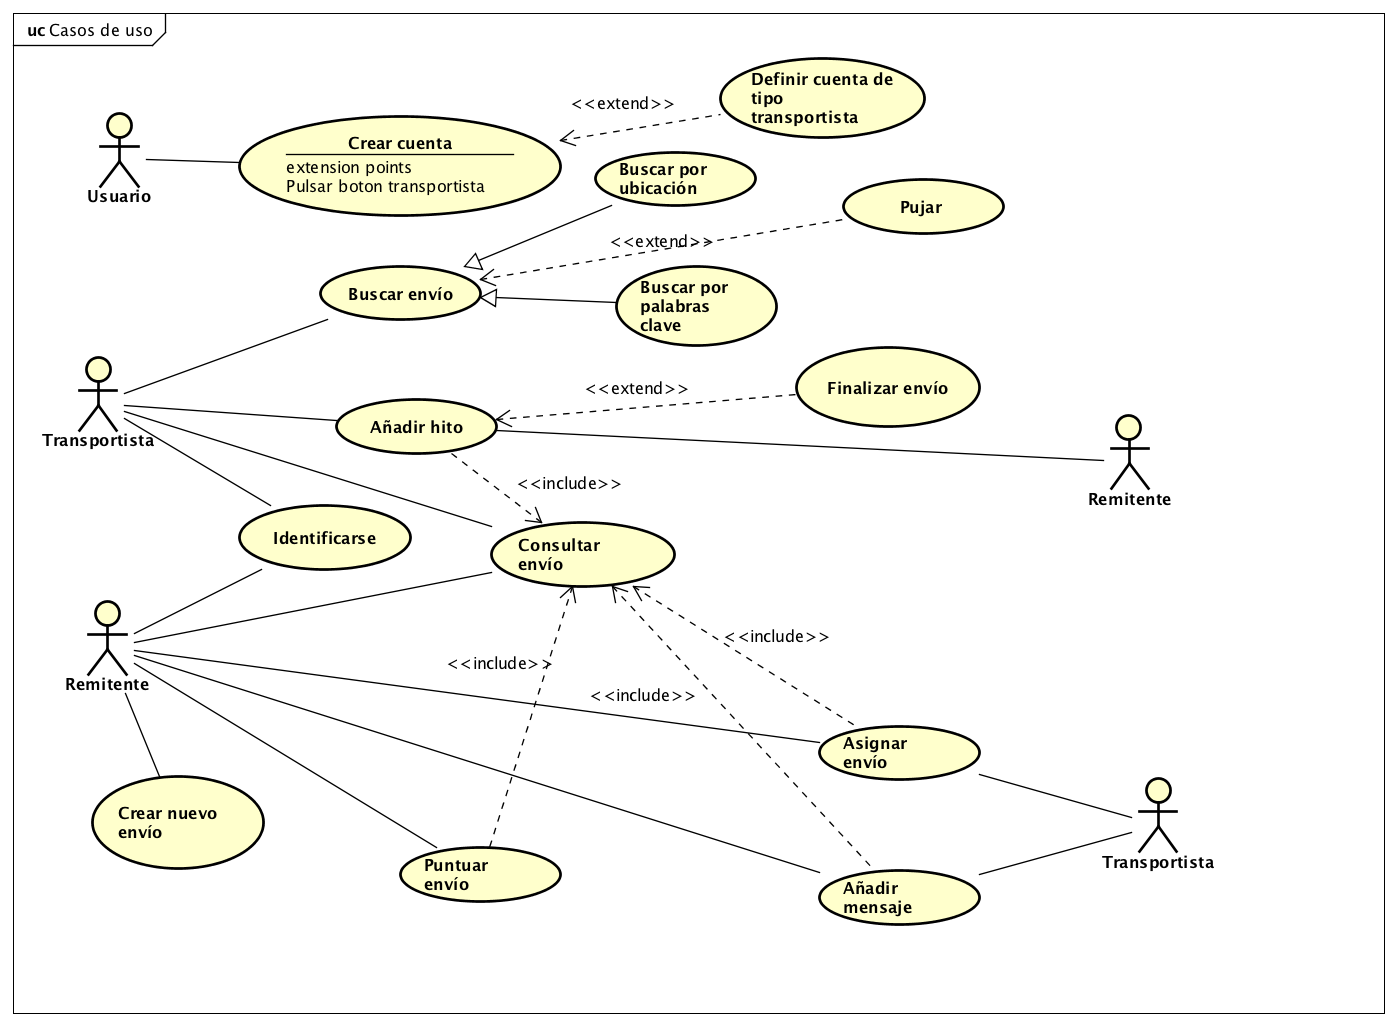
\includegraphics[width=\textwidth]{astah/casos_de_uso.png}
		\end{figure}

		\begin{figure}[H]
			\centering
				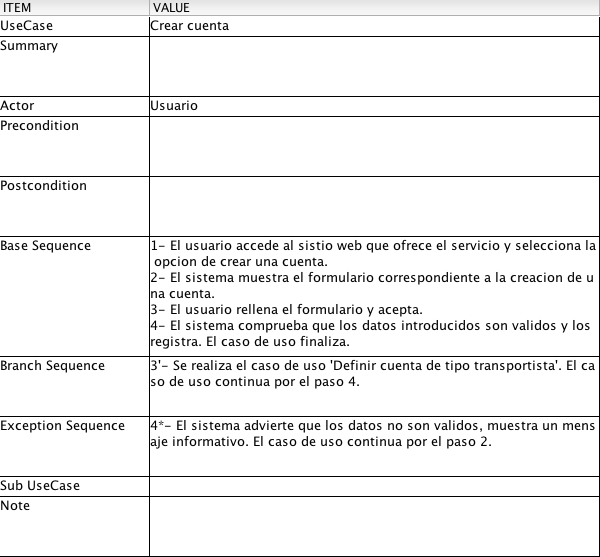
\includegraphics[width=0.75\textwidth]{astah/use_case_crear_cuenta.png}
		\end{figure}

		\begin{figure}[H]
			\centering
				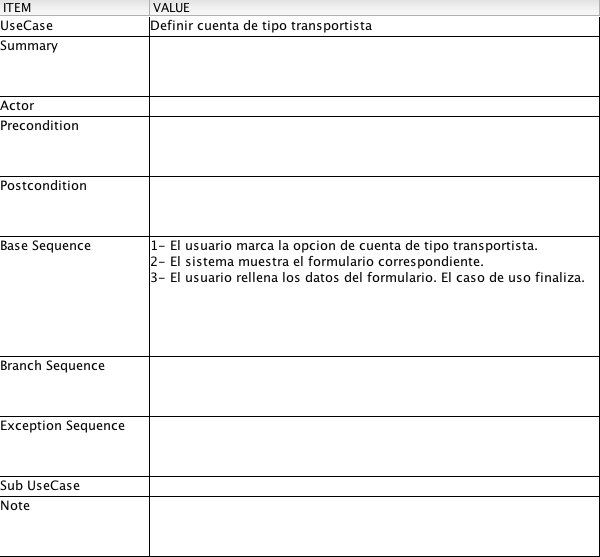
\includegraphics[width=0.75\textwidth]{astah/use_case_definir_transportista.png}
		\end{figure}

		\begin{figure}[H]
			\centering
				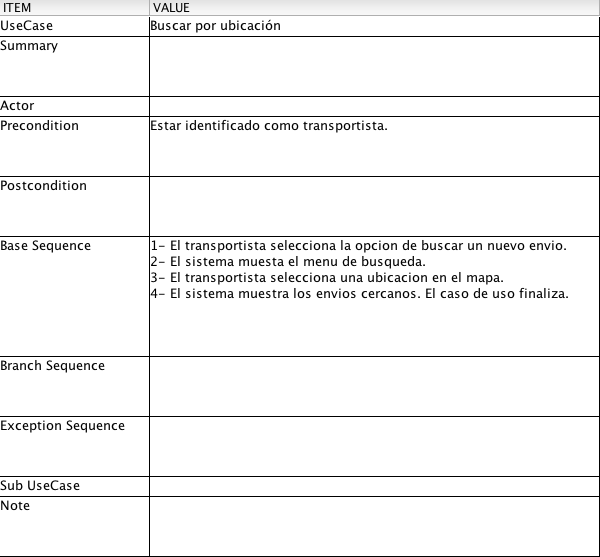
\includegraphics[width=0.75\textwidth]{astah/use_case_buscar_ubicacion.png}
		\end{figure}

		\begin{figure}[H]
			\centering
				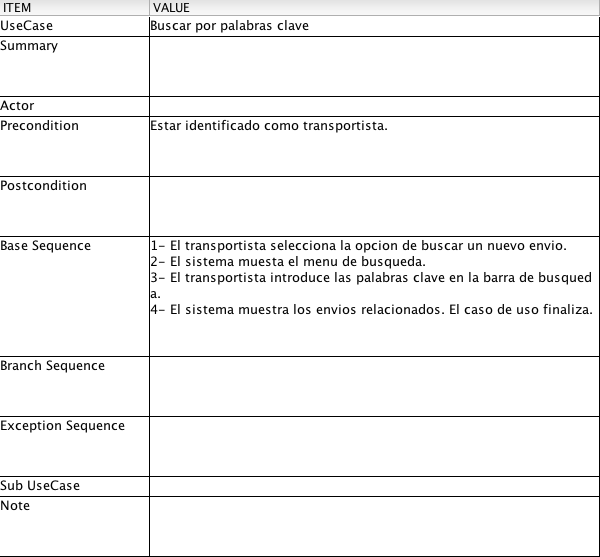
\includegraphics[width=0.75\textwidth]{astah/use_case_buscar_palabras_clave.png}
		\end{figure}

		\begin{figure}[H]
			\centering
				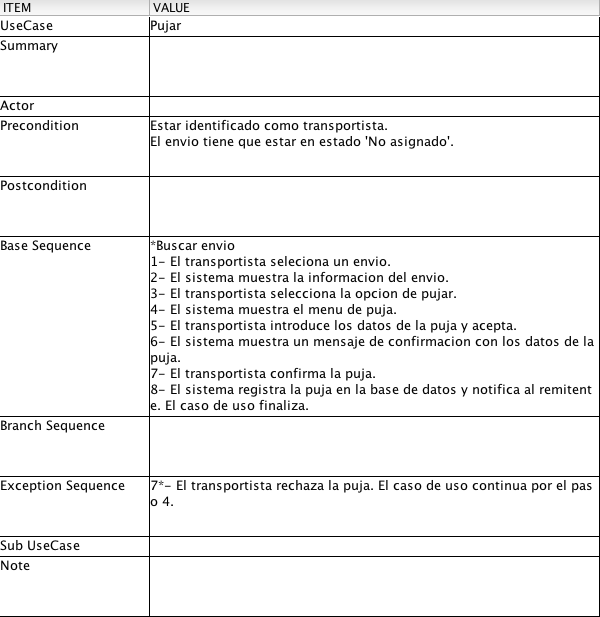
\includegraphics[width=0.75\textwidth]{astah/use_case_pujar.png}
		\end{figure}

		\begin{figure}[H]
			\centering
				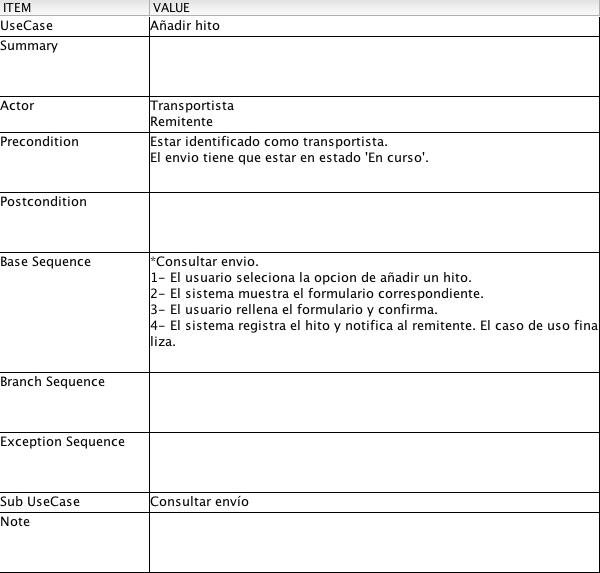
\includegraphics[width=0.75\textwidth]{astah/use_case_anadir_hito.png}
		\end{figure}

		\begin{figure}[H]
			\centering
				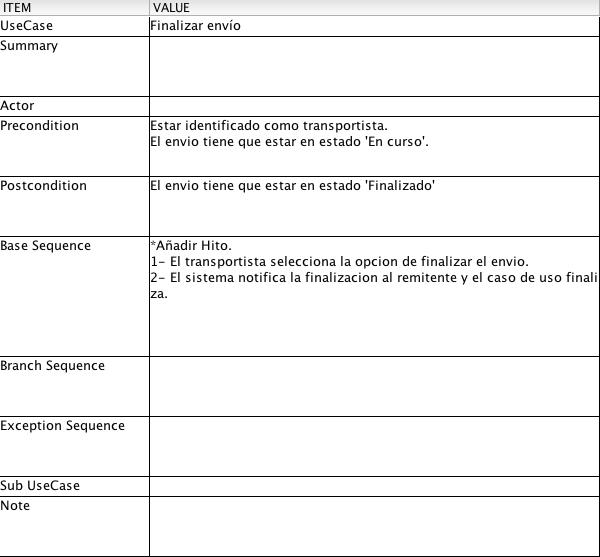
\includegraphics[width=0.75\textwidth]{astah/use_case_finalizar_envio.png}
		\end{figure}

		\begin{figure}[H]
			\centering
				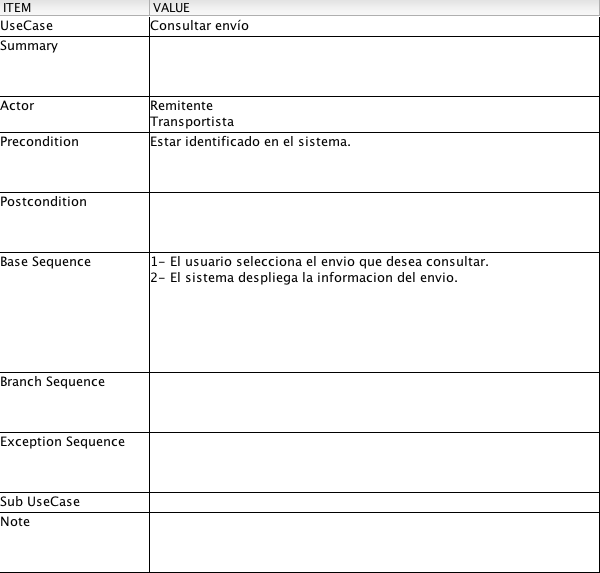
\includegraphics[width=0.75\textwidth]{astah/use_case_consultar_envio.png}
		\end{figure}

		\begin{figure}[H]
			\centering
				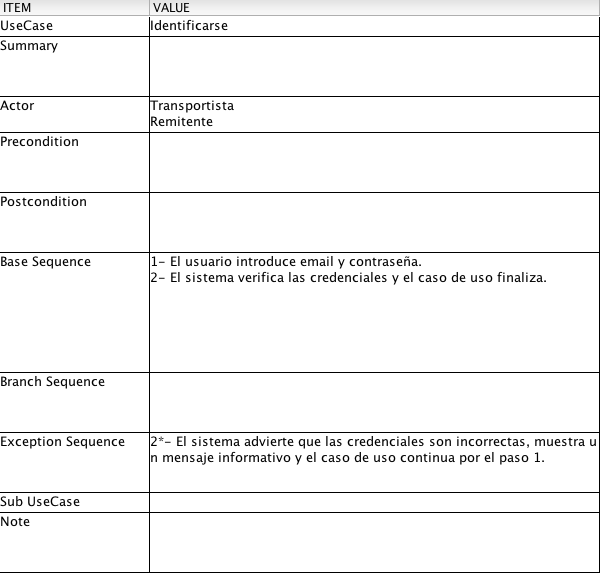
\includegraphics[width=0.75\textwidth]{astah/use_case_identificarse.png}
		\end{figure}

		\begin{figure}[H]
			\centering
				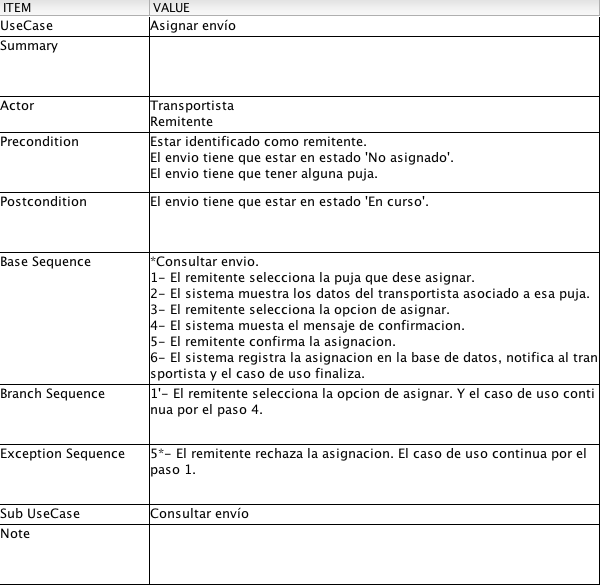
\includegraphics[width=0.75\textwidth]{astah/use_case_asignar_envio.png}
		\end{figure}

		\begin{figure}[H]
			\centering
				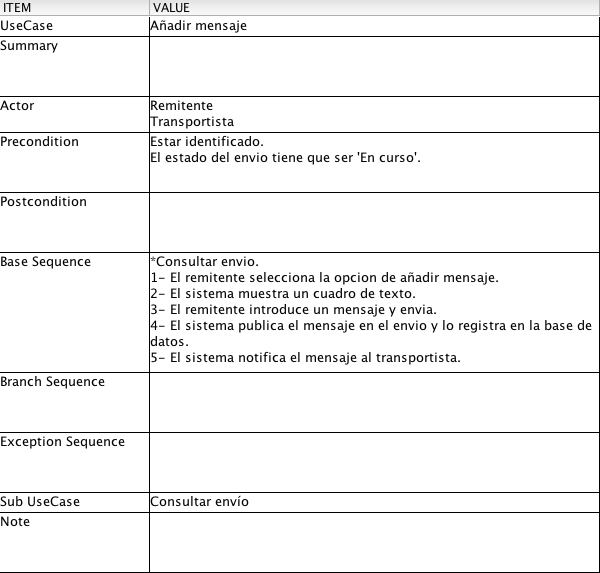
\includegraphics[width=0.75\textwidth]{astah/use_case_anadir_mensaje.png}
		\end{figure}

		\begin{figure}[H]
			\centering
				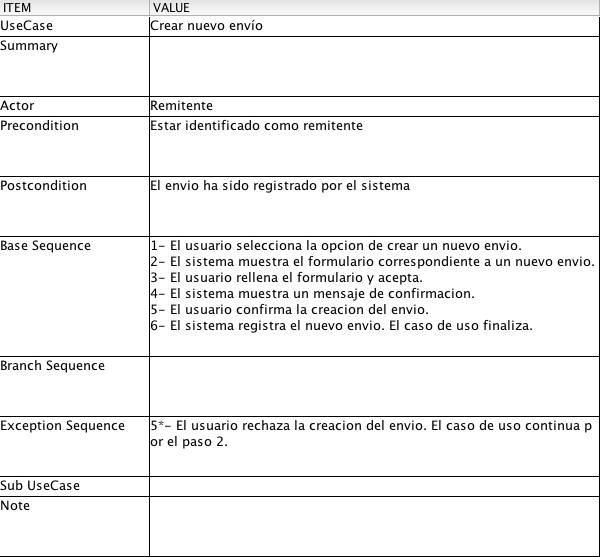
\includegraphics[width=0.75\textwidth]{astah/use_case_crear_envio.png}
		\end{figure}

		\begin{figure}[H]
			\centering
				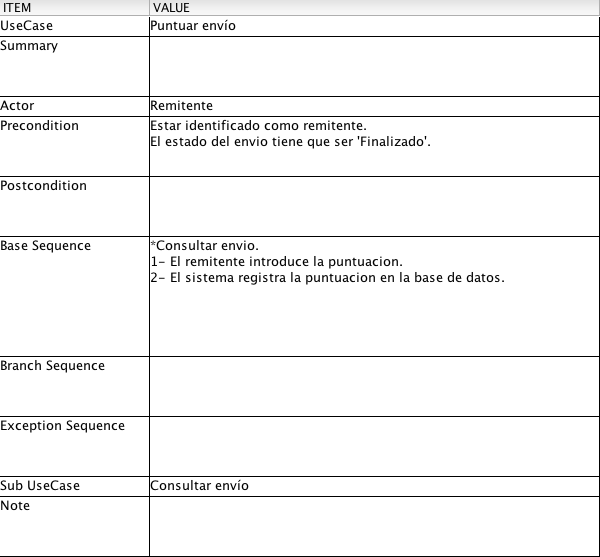
\includegraphics[width=0.75\textwidth]{astah/use_case_puntuar.png}
		\end{figure}

	\section{Modelo del dominio:}

		\begin{figure}[H]
			\centering
				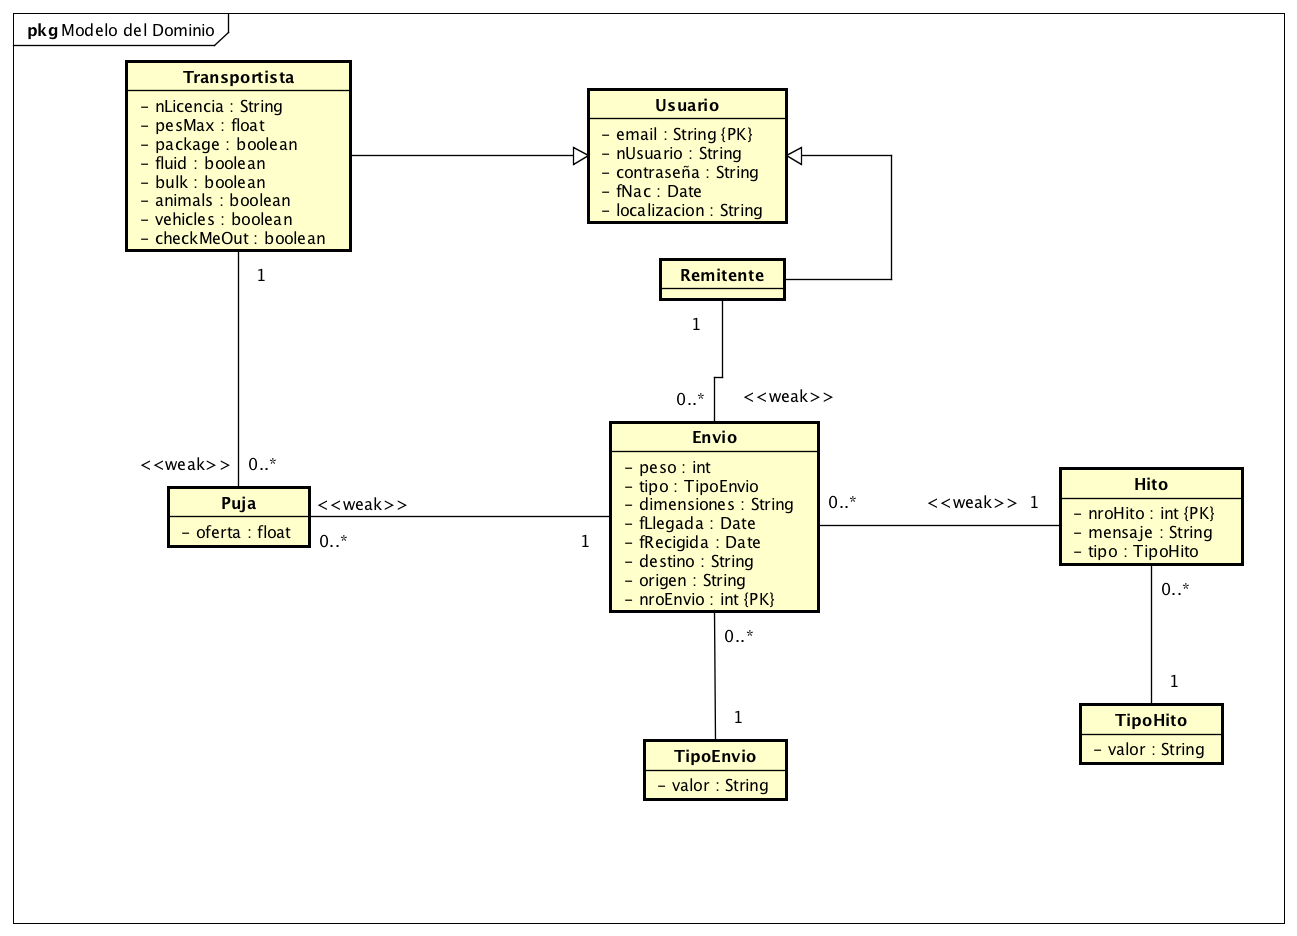
\includegraphics[width=\textwidth]{astah/entidad_relacion.png}
		\end{figure}


	\section{Análisis de los usuarios:}

		\paragraph{}
		Los usuarios que utilizarán el sistema se dividen en dos grupos bien diferenciados, los que lo utilizarán como herramienta para encontrar "ofertas de trabajo", es decir, los \textbf{transportistas}, y los que lo utilizarán como un servicio de mensajería, es decir, los \textbf{clientes}.

		\paragraph{}
		Una vez determinada esta dicotomía pasaremos a describir los 4 perfiles de usuarios objetivo a los cuales está dirigido el sistema:

		\begin{itemize}
			\item \textbf{Transportista Veterano:} \\
				Este perfil de usuario se caracteriza por representar a los trabajadores que han invertido la mayor parte de su etapa laboral en este sector, es decir, conocen bien cómo funciona y no quieren que les "enseñen" a hacer su trabajo. Se localizan en un rango de edad medio-alto (35-55 años). El nivel medio de estudios es básico. Este grupo de usuarios no está muy familiarizado con las nuevas tecnologías y por tanto requiere que el uso de estas sea lo más intuitivo posible. A pesar de estas dificultades se deciden a probar el sistema buscando una mayor cuota de transportes que por otras vias como agencias de transportes. A pesar de ello son bastante incrédulos con las ventajas que esperan recibir al usar el sistema. \\ \\
				\textit{Persona Ficticia: Paco es un camionero de 48 años cuya experiencia laboral se reduce al sector del transporte. Hasta ahora había dependido de una agencia de transportes que le planificaba los envíos pero debido a recomendaciones de compañeros del sector más jóvenes se ha decidido a probar el sistema aunque no está demasiado convencido de sus resultados.}

			\item \textbf{Transportista Fan de las Nuevas Tecnologías:} \\
				Este perfil se diferencia del anterior por englobar a población más jóven (18-35 años) y con un nivel superior de estudios. No tienen miedo a probar nuevas características del sistema y suele gustarles tener una mayor interacción con el cliente. Debido a estas características también son mucho más críticos con el sistema, quejándose mucho más por los fallos o situaciones anómalas que puedan surjir. La motivación que les lleva a utilizar el sistema es el aumento de satisfacción y eficiencia al realizar su trabajo lo cual buscan en un sector tan sacrificado como el del transporte. \\ \\
				\textit{Persona Ficticia: Juan es un chico de 21 años. Obviamente como todo joven de hoy en día no tiene dificultades para manejarse con sistemas informáticos. Tras terminar el bachillerato se ha estado preparando para obtener la licencia de transportista. Recientemente por fin obtuvo el título y con unos ahorros se ha comprado una furgoneta de segunda mano. A pesar de no haber trabajado nunca tiene mucha motivación y ha decidido fijarse en el sistema para probar suerte por primera vez.}

			\item \textbf{Cliente para uso Empresarial:} \\
				A diferencia de los anteriores, este perfil de usuario ve el sistema como un servicio de mensajería en vez de como una herramienta de trabajo. Además estos clientes no utilarán el sistema para beneficio propio, sino en nombre de una empresa, es decir, podrían ser trabajadores de un departamento de logística. El rango de edad en este caso es muy amplio ya que probablemente no usarán el sistema por su propia voluntad, sino porque se lo impone su empresa. El nivel de estudios de este grupo de usuarios es alto y por lo general están familiarizados con el uso de las nuevas tecnologías. Están muy interesados en la visualización de estadísticas sobre envíos recibidos y envíados para tratar de optimizar y reducir costes en futuros envíos.\\ \\
				\textit{Persona Ficticia: Cristina es una trabajadora de una gran empresa del sector automovilístico. Trabaja en una de sus filiales en el departamento de logistica por lo cual tiene que gestionar envíos entre diferentes filiales y concesionarios. La empresa en la que trabaja quiere reducir sus costes por lo que ha decidido empezar a usar progresivamente el sistema y promete confiar todo su flujo de envíos en él si los resultados son los esperados.}

			\item \textbf{Cliente para uso Personal:} \\
				Este grupo de usuarios se caracteriza por ser el único grupo de usuarios que usa el servicio para fines personales. En este grupo se encuentran personas jóvenes que no tienen miedo a sufrir riesgos (ya que por lo general personas de una edad más avanzada son reacios a utilizar sistemas de este tipo por miedo a que su mercancia no llegue al destino). Utilizan las nuevas tecnologías a diario y por ello están familiarizados con servicios similares. El nivel de estudios de este grupo es muy variado. La motivación a la hora de usar el sistema es la facilidad que proporciona un servicio online frente a la alternativa clásica del servicio de mensajería, además de que esperan un menor coste.\\ \\
				\textit{Persona Ficticia: Ana es una joven de 26 años que tras haber estado trabajando desde hace unos años por fin ha conseguido reunir el dinero suficiente como para comprarse un coche. Debido a esto la ha surgido la dificultad de cómo recibirlo ya que la marca que ha elegido no tiene un concesionario en su ciudad y el más cercano no se hace cargo de este problema. Ana recuerda que hace poco vió un anuncio en la televisión sobre un nuevo sistema de transportes que cree que podría ayudarla con dicho problema.}

		\end{itemize}


	\section{Escenarios del sistema futuro:}

		\paragraph{}
		Los escenarios expuestos para el sistema son los siguientes:

		\begin{itemize}
			\item \textbf{Escenario 1:} \\
				Miguel es un camionero que ha oido hablar del sistema, por lo que se decide probar su funcionamiento dado que ha oido muy buenos comentarios sobre él. Nunca antes lo había probado, por lo que crea una cuenta en el sistema indicando que es transportista. Para ello introduce sus datos personales, además del número de licencia de transporte y las características de la mercancía que es capáz de transportar. Una vez creada la cuenta lo siguiente que hace en el sistema es buscar envíos. Para ello introduce su localización actual y el sistema le muestra un listado de las envíos que puede realizar, ofreciendole la posibilidad de pujar por ello. Dado que Miguel quiere probar el sistema se decide a pujar por unos cuantos envíos para probar la utilidad del sistema. Una vez hecho esto, tendrá que esperar hasta que alguna de las pujas sea aceptada.

			\item \textbf{Escenario 2:} \\
				Teresa es una usuaria habitual del sistema, el cuál utiliza para envíar cosas a su familia y amigos dado que le ofrece la facilidad de poder realizar todos los trámites online. Teresa ha decidido mudarse de casa el próximo mes, para lo que utilizará el sistema para trasladar todos sus bienes a su nueva casa. Lo que hará será por tanto crear un nuevo envío para lo cual tendrá que introducir las direcciones de origen y destino así como el tamaño y peso aproximados del envío. Una vez hecho esto espera a que algún transportista ofrezca una puja sobre el envío. En el momento en el que encuentre un precio que esté dispuesta a aceptar y las valoraciones del transportista la convenzan aceptará dicha puja. Durante todo el proceso de envío tanto el transportista como ella podrá interactuar a través de hitos y comentarios sobre el transporte. Una vez finalizado el envío Teresa podrá introducir una valoración acerca del transportista que después otros usuarios podrán visualizar en el momento de aceptar las pujas.

			\item \textbf{Escenario 3:} \\
				Oscar acaba de comprar una nueva consola a través de internet. La web a través de la cual ha realizado la compra utiliza el sistema para llevar a cabo el transporte, por lo cual le ha enviado un enlace para que pueda monitorizar el proceso. Dado que Oscar todavía no tiene una cuenta en el sistema lo primero que hará será registrarse en el mismo introduciendo sus datos personales, pero omitiendo seleccionar que es un tranportista. Una vez hecho esto podrá consultar su envío a la vez que introducir hitos y comentarios sobre él, que tanto el transportista que lo traslade como el remitente (en este caso la web) podrán visualizar. Una vez finalizado el envío Oscar podrá valorar al transportista.

		\end{itemize}


	\section{Mapa del sitio:}


		\begin{figure}[H]
			\centering
				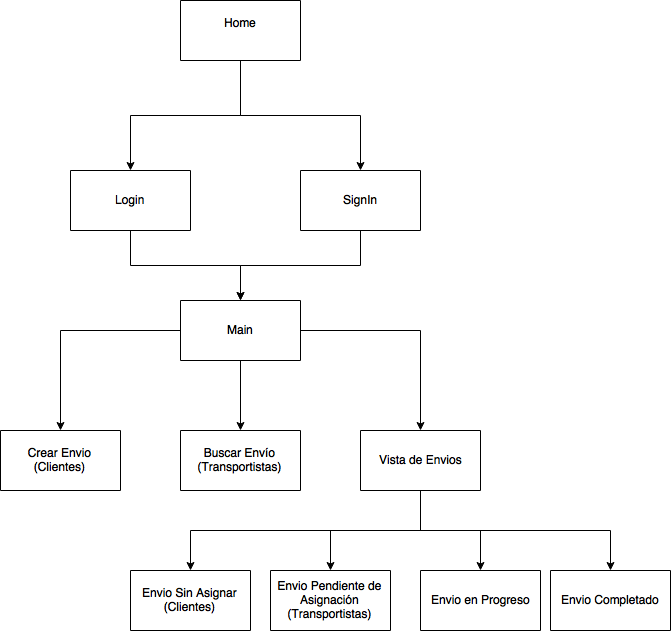
\includegraphics[width=0.75\textwidth]{sitemap.png}
		\end{figure}

	\section{Guía de Uso}

		\paragraph{}
		Dado que la página web está hecha con Angular.js y se ha utilizado una única página raíz en la cual se van incluyendo las distintas partes según convenga, para probar la página hay que ejecutar \textbf{web/index.html}.

		\paragraph{}
		En esta primera vista podemos encontrar dos botones azules, que sirven para crearse una cuenta e iniciar sesión en el sistema. Al no tener que implementar la funcionalidad del sistema (aunque buena parte ha sido adelantada), se han habilitado dos botones verdes de muestra para poder simular los casos de hacer login con una cuenta de transportista y de cliente.

		\paragraph{}
		La página de inicio es muy similar para efectos del transportista y del cliente. En esta vista podemos encontrar los envíos en los que cada uno está participando, con dos diferencias notables:

		\begin{enumerate}
				\item Para los envios sin asignar, los transportistas tienen la etiqueta \textbf{pendiente} mientras que los clientes tienen \textbf{no asignado}.
				\item En la barra superior el cliente tiene la opción de elegir la opción \textbf{crear envío}, desde la que accederá al menú modal con el formulario para solicitar un envío. El transportista, sin embargo, podrá hacer uso de la opción \textbf{buscar envío}, en la que le aparecerán los envíos sobre los que puede pujar.
		\end{enumerate}

		\paragraph{}
		\textit{Importante}: Para probar las distintas funcionalidades del cliente y el transportista, \textbf{cerrar sesión} en vez de usar el botón de atrás del navegador. Esta opción se encuenta pulsando en el nombre del usuario de la esquina superior izquierda.

		El desarrollo de esta web ha sido probado con los siguientes navegadores web: Mozilla Firefox, Google Chrome (ejecutando desde un servidor, por políticas de seguridad) y Safari.


	\section{Casos de uso implementados}

		\paragraph{}
		Para comprobar estas funcionalidades se debe crear y poblar la base de datos con los scripts de creación y población de la base de datos que están en la carpeta database/.

		\paragraph{}
		Implementación de la solicitud de ingreso en el sistema, con su correspondiente acceso a la base de datos y el sistema de tokens para mantener la sesión del usuario conectado. (Las credenciales se pueden ver en el script de población de la base de datos, en la tabla Usuario).

		\paragraph{}
		Creación dinámica de la lista de envios asociados a un usuario. En este caso, aparecerán para el remitente los que se han insertado por defecto en el script de población.

		\paragraph{}
		Añadir hitos a los diferentes envios. Se pueden insertar en la base de datos nuevos hitos y dinámicamente se actualizan en la tabla principal de envios.
    \section{Descripción de la estructura de la base de datos}

    		\paragraph{}
		En la figura adjunta se muestra el esquema de las tablas resultantes del modelo E/R, con todos sus atributos, subrayadas las claves primarias y marcadas con flechas las claves ajenas.

		\paragraph{}
		A continuación se exponen las justificaciones oportunas sobre las que se basa el diseño de estas tablas:
		\begin{enumerate}
			\item Las tablas TipoHito, TipoEnvio y TipoEstado sirven para almacenar todos los códigos de este tipo de operaciones. Es decir, al existir solo cuatro tipos de envíos, en TipoEnvio se guardan las definiciones de estos cuatro tipos y desde las tablas que las referencian se puede conocer estos valores por el código, sin necesidad de almacenar de nuevo el nombre del tipo.
			\item Transportista y Remitente son especializaciones de Usuario, por lo que sobre esta última se almacena la infomación común a ambas y mediante las dos primeras se puede conocer qué tipo de usuario es cada uno a partir del email.
			\item Para conseguir los envios a los que está asociado un Transportista, es necesario usar el enlace con la tabla Puja. Esto es así porque los envios de los transportistas son referencias a los envios que un Remitente ha creado, luego habría que replicar el envío varias veces si se almacenase dentro de la tabla Envio. Esto nos proporciona una mejor gestión del espacio de almacenamiento..
		\end{enumerate}

		\begin{figure}[H]
			\centering
				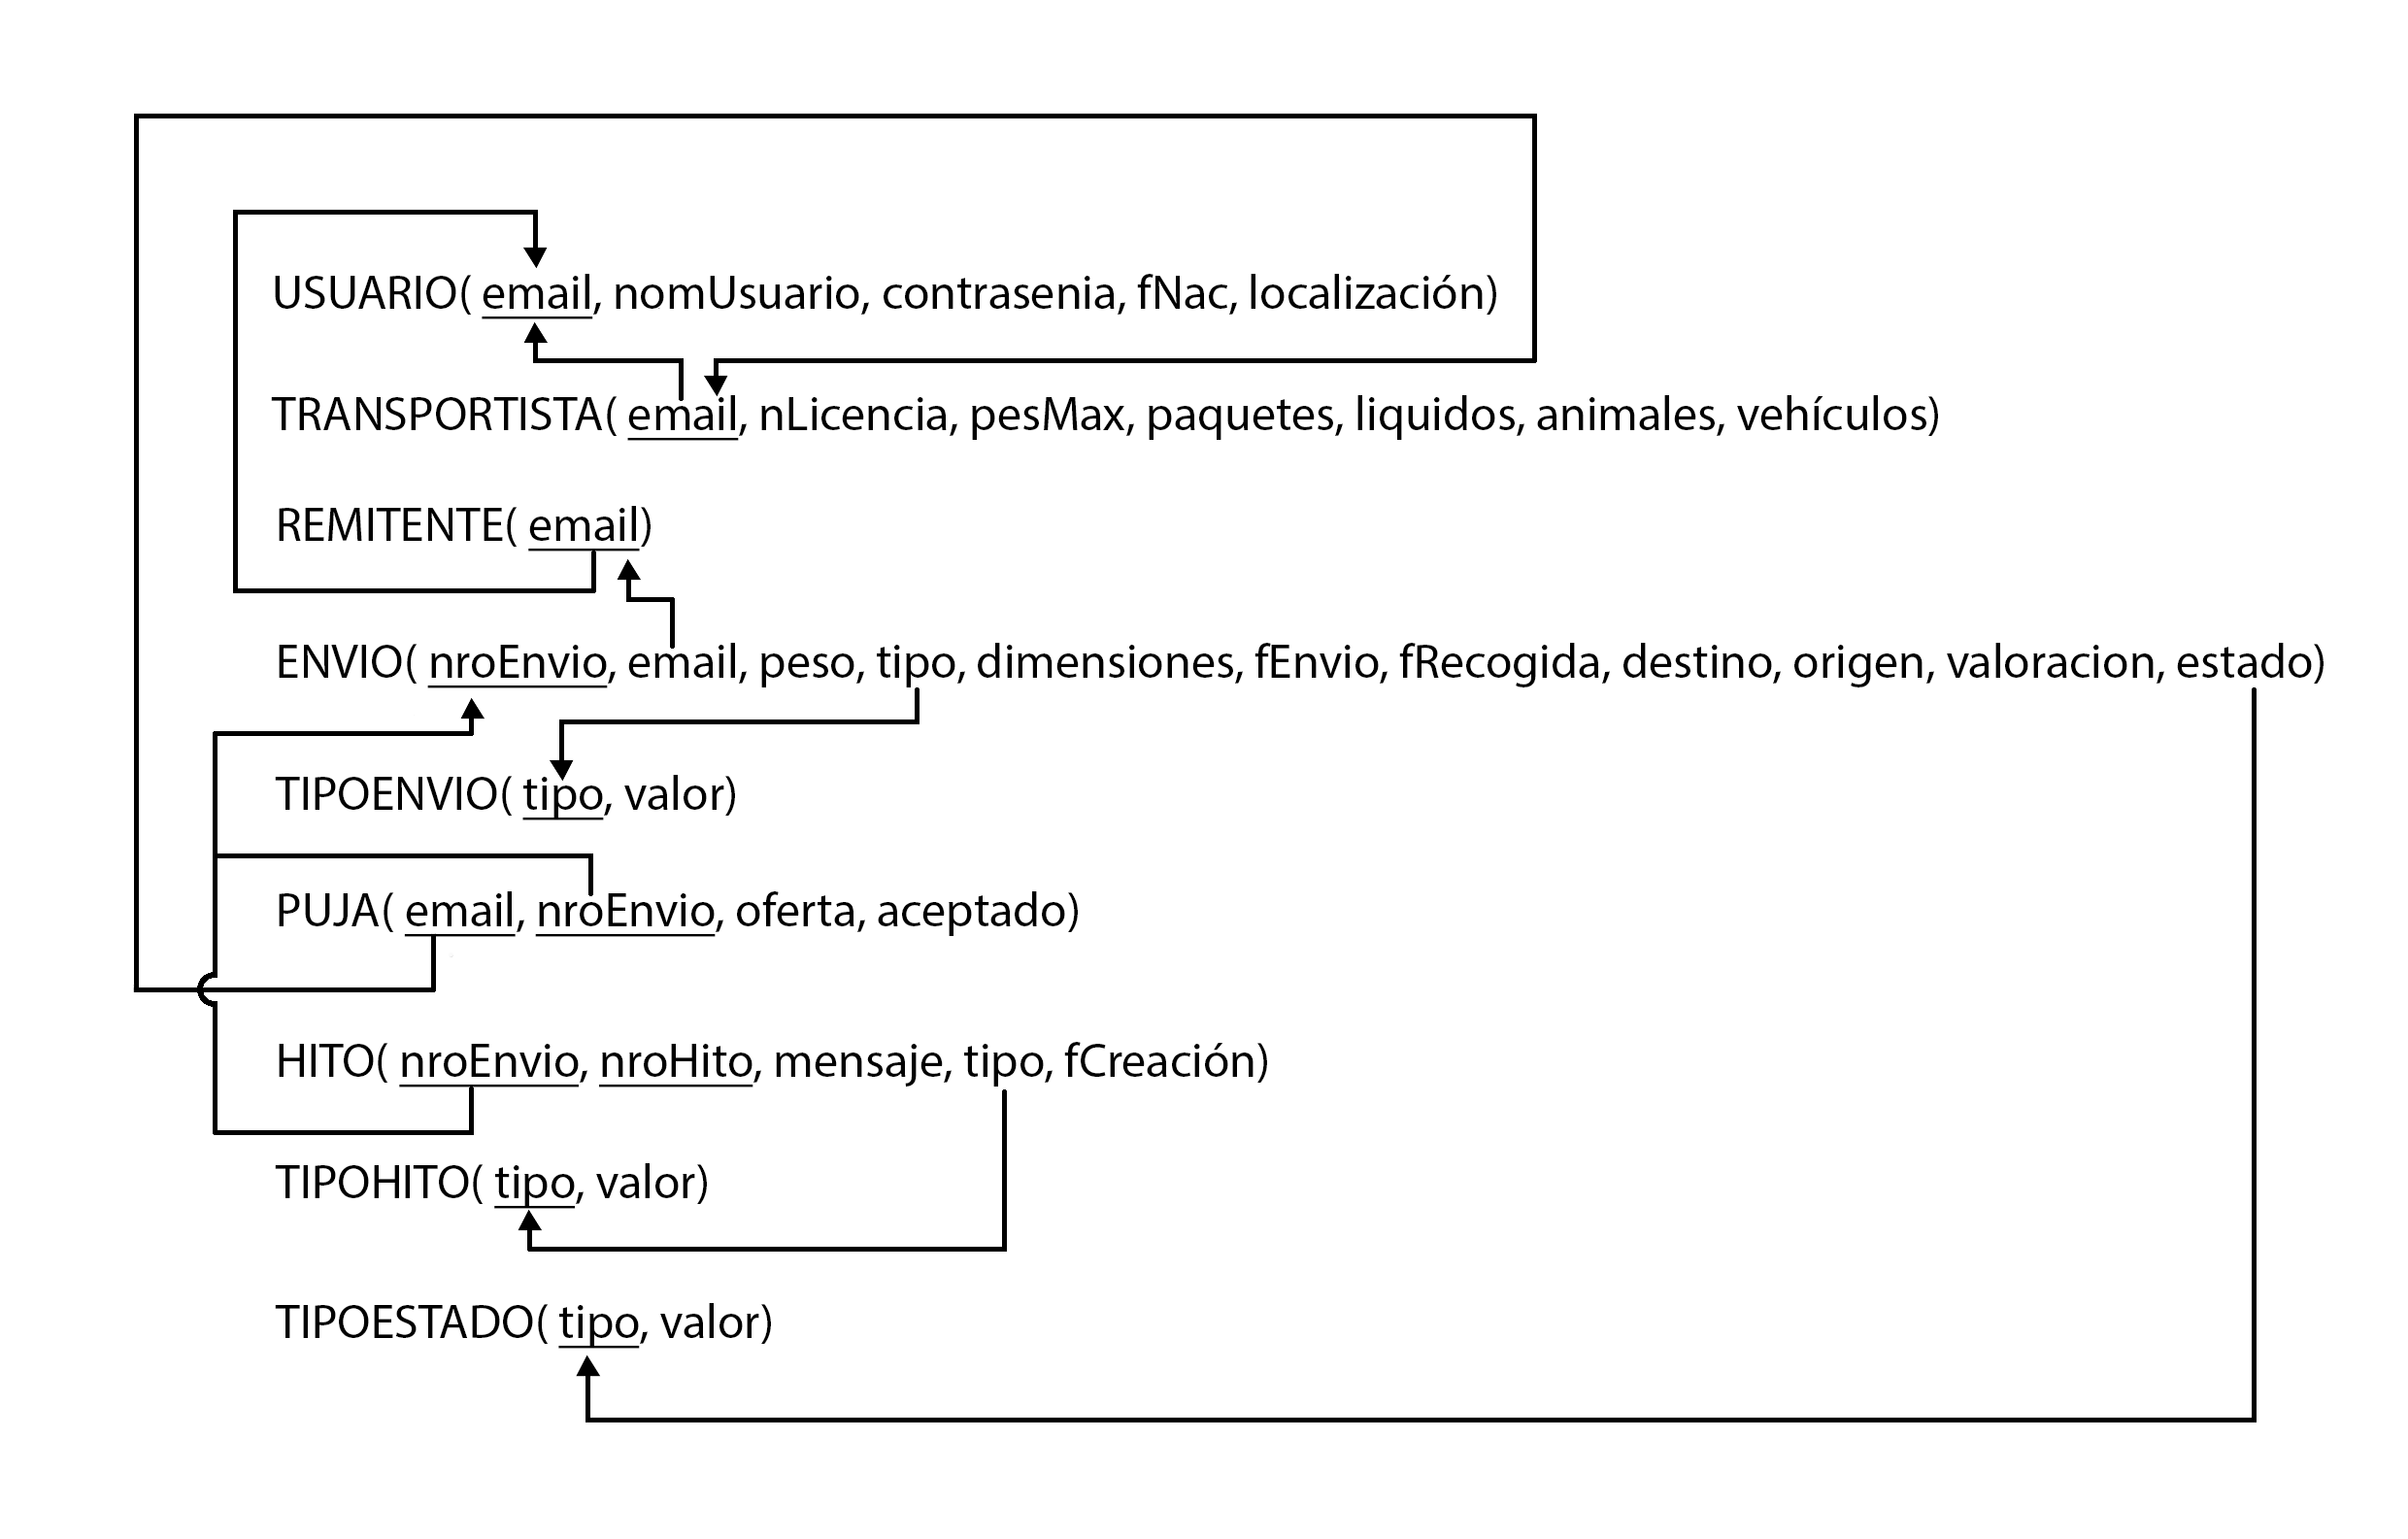
\includegraphics[width=1\textwidth]{database.png}
		\end{figure}
%----------------------------------------------------------------------------------------
%	Bibliographic references
%----------------------------------------------------------------------------------------
	\begin{thebibliography}{9}

		\bibitem{wikipedia_transporte}
		Wikipedia. Transporte. \url{https://es.wikipedia.org/wiki/Transporte}

		\bibitem{expansion_uber_transporte}
		Expansión. Se busca el Uber del transporte de mercancías. \url{http://www.expansion.com/economia-digital/2015/10/29/5630ef8e46163f932a8b45d9.html}

	\end{thebibliography}

\end{document}
